\documentclass{article}
\usepackage[a4paper, margin=2.5cm]{geometry}
\usepackage{amsmath}
\usepackage{caption}
\usepackage{placeins}
\usepackage{graphicx}
\usepackage{subcaption}
\usepackage{setspace}
\usepackage{float}

%\usepackage[active,tightpage]{preview}
\usepackage{natbib}
\bibpunct{(}{)}{,}{a}{}{;} 
\usepackage{url}
\usepackage{nth}
\usepackage{authblk}
% for the d in integrals
\newcommand{\dd}{\; \mathrm{d}}
\newcommand{\tc}{\quad\quad\text{,}}
\newcommand{\tp}{\quad\quad\text{.}}
\defcitealias{HMD}{HMD}

\newcommand\ackn[1]{%
  \begingroup
  \renewcommand\thefootnote{}\footnote{#1}%
  \addtocounter{footnote}{-1}%
  \endgroup
}
\begin{document}

%\title{Macro patterns in the shape of aging}
\title{Spell analysis in multistate Markov models}
\author[1]{Tim Riffe\thanks{riffe@demogr.mpg.de}}
\affil[1]{Max Planck Institute for Demographic Research}
\maketitle

\begin{abstract}
Multistate matrix population models are typically used to compute statistics
such as the state occupancies or the moments thereof. Recently formulas
have been derived to compute the average number of spells for a given state,
which combined with the average state occupancy yields the average spell
duration. I've since wondered what the age pattern to average spell durations
is. Here I demonstrate how to use simulations to estimate a variety of age and
other patterns of different state spells. 
\end{abstract}

\section{Introduction}
The amount of population-level measures that one might devise for a particular
population-level process is dizzying, so it may beg the question from the outset
why we might desire to have more. Matrix-based manipulations of incidence-based
models are rather undeveloped with respect to tenure-statistics, and these might
be of interest for a variety of substantive reasons. By tenure statistics I
refer to the statistics of particular spells or episodes of a state. Namely, in
incidence-based models with bidirectional flows (i.e. allowing for recovery and
then re-onset, and so on), a hypothetical individual may pass through a state
(say sickness) many times before death. Typically a transition matrix
manipulation would only give us the average time spent sick (or moment
statistics thereof). Recently matrix calculations have been described for how to
calculate the average number of episodes of a given state \citep{dudel2017b}.
Combined with the average state occupancy, this information yields the average
duration of episodes.

One may wonder how the average spell duration changes with age, and for this
there is no ready matrix expression (although it would of course be possible). I
will procede using simulations rather than matrix calculations because it will
save the work of deriving and checking dozens of formulas. In this way, we have
the liberty to change definitions without incuring methodological setbacks.
Since we simulate, we get stochastic stationary distributions of each
measurement, which I'll represent using fan-chart visualizations. This approach is not all that different from
that proposed by \citet{laditka1998new}, but I take things a bit
farther by proposing a suite of age realignments and resulting age-like patterns of episode
statistics. 

\section{Data}
The point of departure for all calculationsis a
transition matrix. To demonstrate, I use a published transition matrix from a recent
study of working life expectancy in the United States \citep{Dudel2017}. This
matrix refers to black females aged 50-100 in 1994. The same sorts of things can
be done with any age-stage matrix. Actually technically you could do the same with
an ageless matrix, if the simulated sequence steps are interpretable as age.

\section{Simulation}
I take advantage of the recently published \texttt{R} package
\texttt{markovchain} \citep{spedicato2017}, which includes a random state
sequence generator function \texttt{rmarkovchain()} that mereley requires a
transition matrix to do its work.\footnote{There are some trivial object
definition steps to convert the employment matrix into a conformable markov
object before feeding it to the random generator.} I generate a large number,
say 10k or more trajectories to operate on as the stationary population. Each
trajectory consists in a \texttt{character} vector of states
[\texttt{Employed},\texttt{Inactive},\texttt{Retired},\texttt{Dead}], where dead
is of course an absorbing state, but the other states can be switched on and off
annually from ages 50 and higher.\footnote{It would also be possible to further
graduate transition rates to standardized month or week units to produce higher
resolution sequences, but this is unnecessary for the present treatment.}

A glimpse of the first 10 randomly generated individuals is shown in
Figure~\ref{fig:seq10}. These ten individuals will be recycled in all of the
following data manipulations used to demonstrate concepts. All aggregate
calculations of age patterns (and so on) are done on the full simulated population. In this case, I simulated
assuming that one starts in a state of employment at age 50, but the starting
state could also easily be a mixture of states.

\begin{figure}[ht!]
\centering
\caption{Ten randomly generated state sequences from the 1994 transition matrix
of black females \citep{Dudel2017}}
\label{fig:seq10}
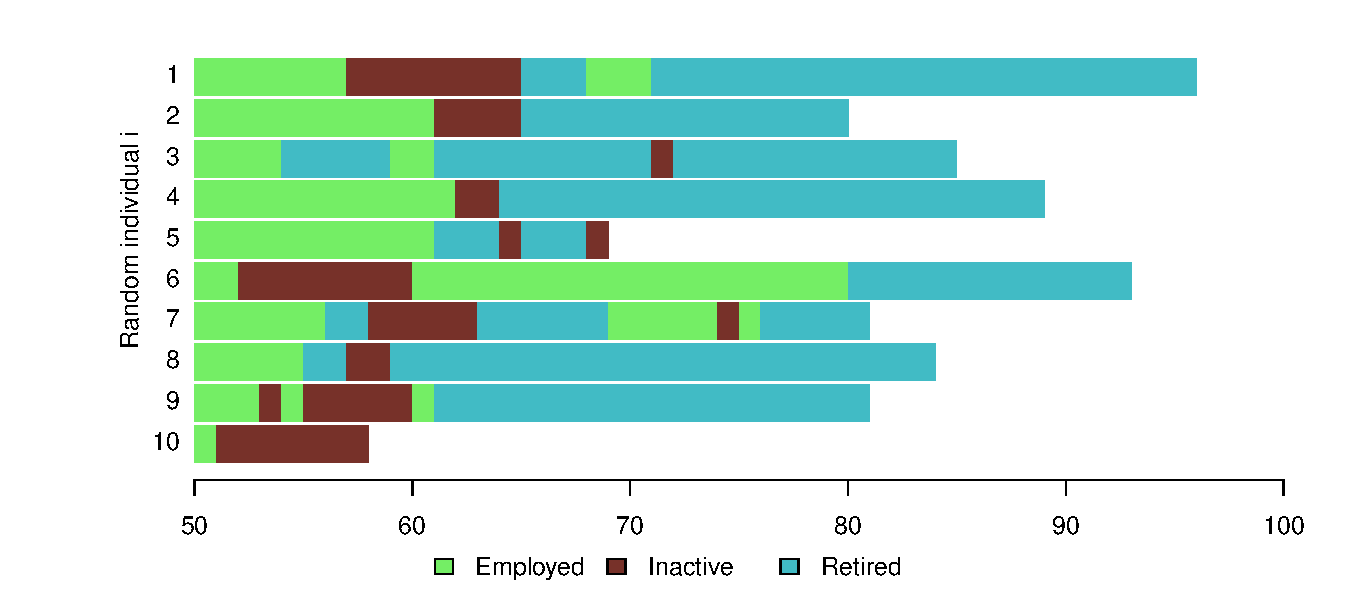
\includegraphics[scale=.5]{Figures/Seq10.pdf}
\end{figure}

Standard calculations of prevalence typically procede by imputing reference
states with 1s (with 0s elsewhere) and taking column means over survivors in
each age. Figure~\ref{fig:seq10ones} shows such a data construct, where the
state sequence matrix has been converted to a binary matrix, with 1s for
employment episodes, 0s for other living states (shown blank). Typically one
might impute NA values in dead states for this sort of calculation. Operations on
objects such as this can yield age patterns of prevalence or
expectancies, for example.

 \begin{figure}[ht!]
\centering
\caption{Binary imputation of employment spells}
\label{fig:seq10ones}
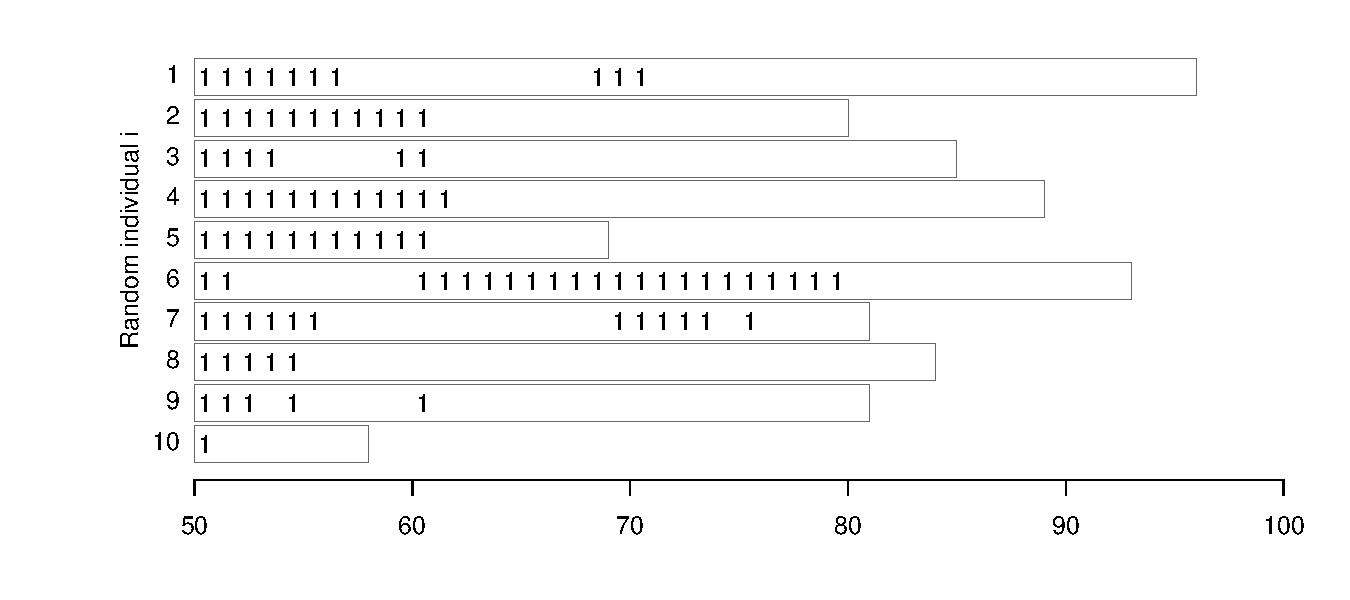
\includegraphics[scale=.5]{Figures/Seq10ones.pdf}
\end{figure}


\FloatBarrier
\section{Running clocks and alignment}
Beyond counting episodes, one may wish to aggregate statistics on each episode
in novel ways. For instance, conditional on being in state $s$ in age $x$, what
is the average duration of spell that one finds oneself in? 

\subsection{Clocks}
To calculate the average spell duration by age, first convert our state
sequences to a data object something like Figure~\ref{fig:seq10dur}. Using chronological age as the reference, one may also wish to calculate time
spent or left in the state episode, per
Figure~\ref{fig:seq10timespent} or \ref{fig:seq10timeleft} \footnote{Actually,
I'd increment values by $\frac{1}{2}$ for mid-state clocking, but decimals would squeeze the figure too
much.}. In either of these cases, value alignment is with respect to episode
entry or exit, but aggregation alignment remains pegged to age. Statistics
across individuals in an array with therefore produce age patterns.

\begin{figure}[ht!]
\centering
\caption{Inactivity spells from Figure~\ref{fig:seq10}
are imputed with different duration count variables. It's probably better to add
$\frac{1}{2}$ to the displayed \emph{running} values. }
\label{fig:spentleft}

\begin{subfigure}{\textwidth}
\caption{Static; Total episode duration of inactivity.}
\label{fig:seq10dur}
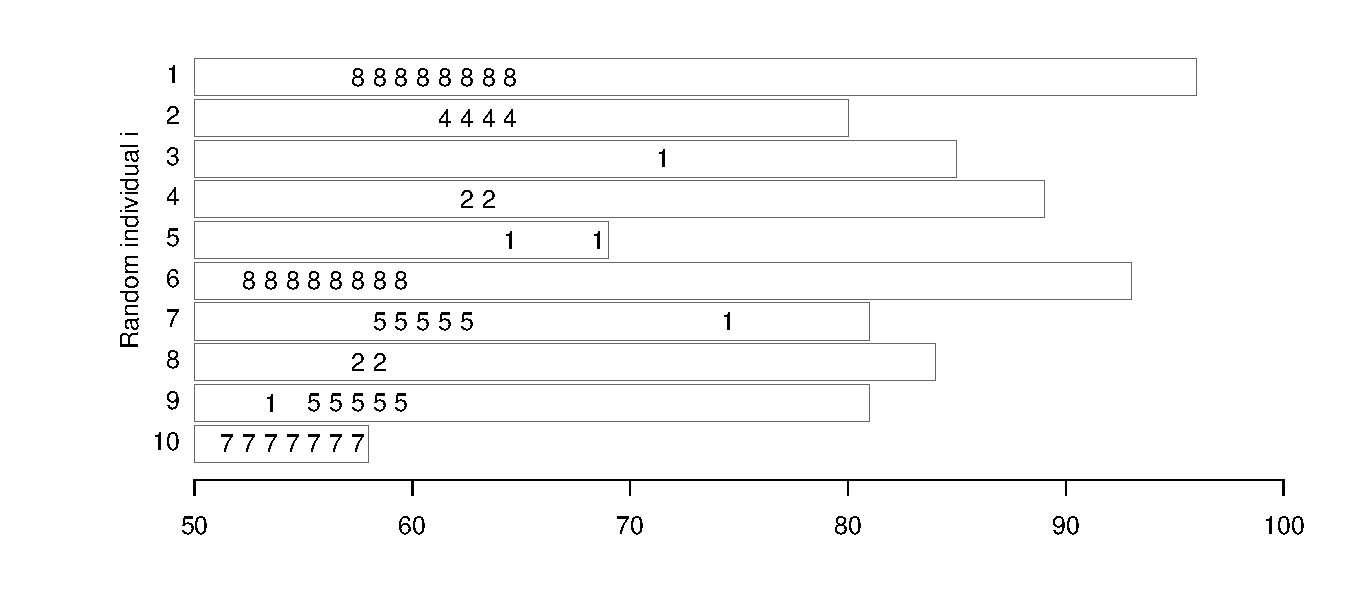
\includegraphics[scale=.5]{Figures/Seq10dur.pdf}
\end{subfigure}

\begin{subfigure}{\textwidth}
\caption{Running; Time spent in episode of inactivity.}
\label{fig:seq10timespent}
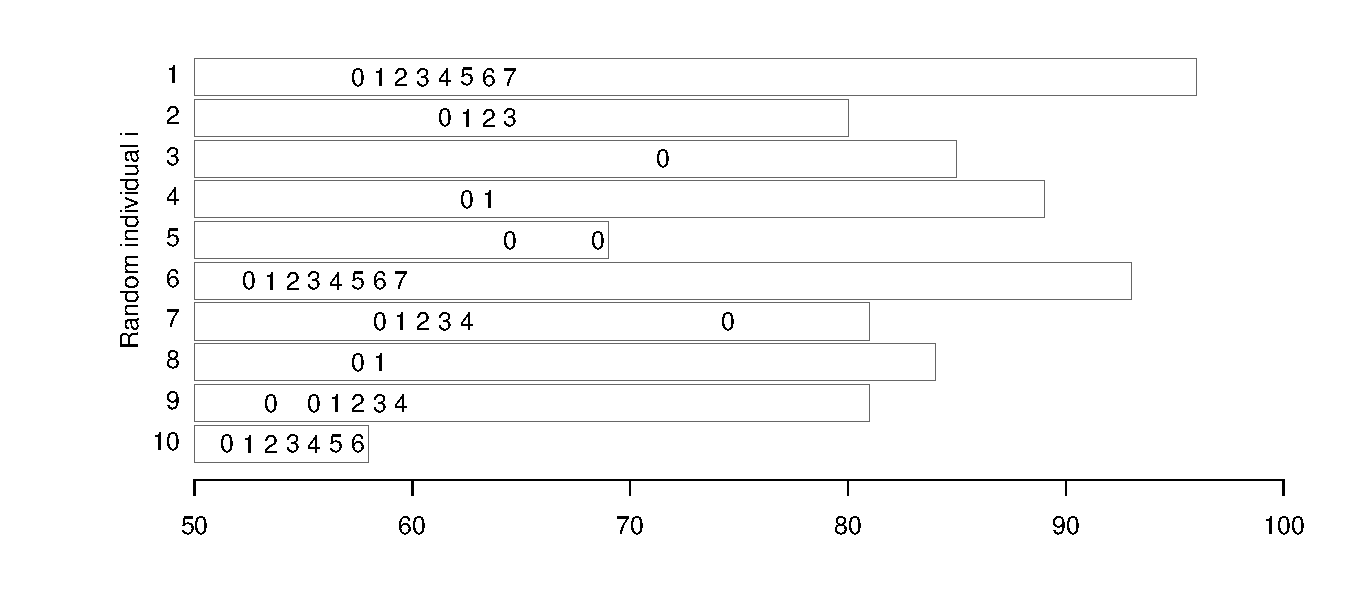
\includegraphics[scale=.5]{Figures/Seq10timespent.pdf}
\end{subfigure}

\begin{subfigure}{\textwidth}
\caption{Running; Time left in episode of inactivity}
\label{fig:seq10timeleft}
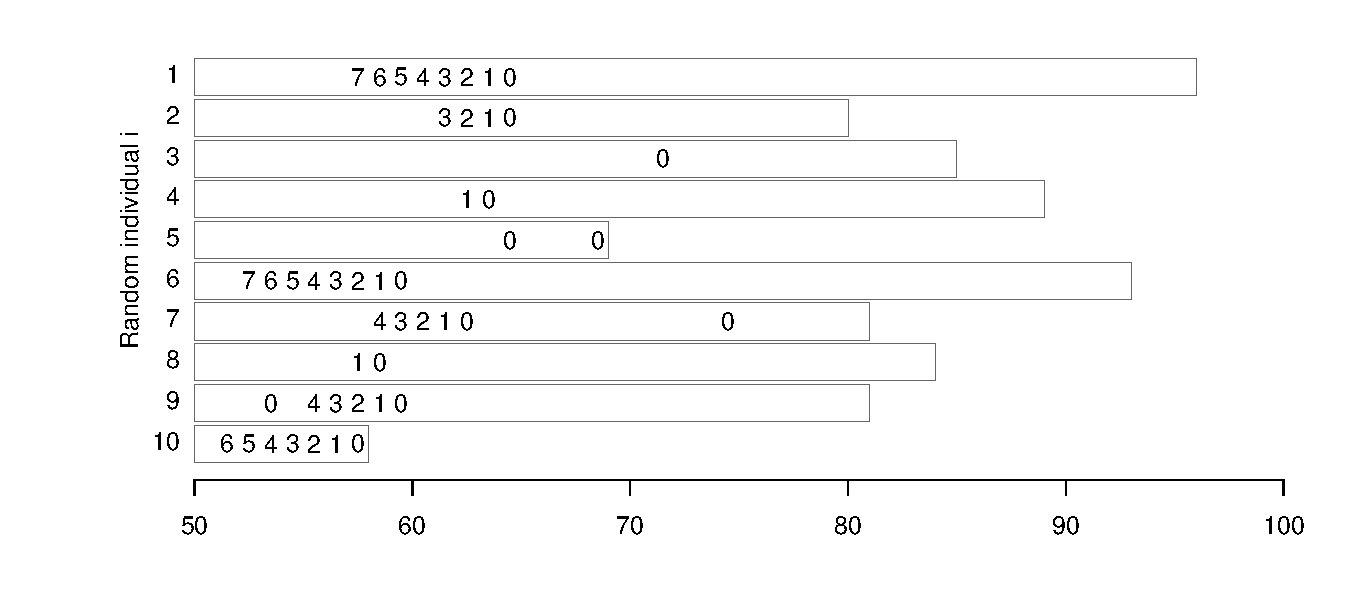
\includegraphics[scale=.5]{Figures/Seq10timeleft.pdf}
\end{subfigure}
\end{figure}

One may fill episodes with other markers, such as episode
order, as in Figure~\ref{fig:order} for the case of employment spells, or
episode fractions. One could further condition age patterns of total duration, time spent, or time left on episode order. If spells are
filled with 1s, then aggregation results in prevalence. Note, time \emph{left}
in the episode has no left-truncation problem, also not in the aggregate. 
These series of values, that I call clocks, are then aggregated in some
way, and aggregation is always within some external structuring classes that
remain to be defined. 

\begin{figure}[ht!]
\centering
\caption{Employment episodes from Figure~\ref{fig:seq10}
are imputed with order count variables.}
\label{fig:order}

\begin{subfigure}{\textwidth}
\caption{Employment episode order, increasing.}
\label{fig:orderup}
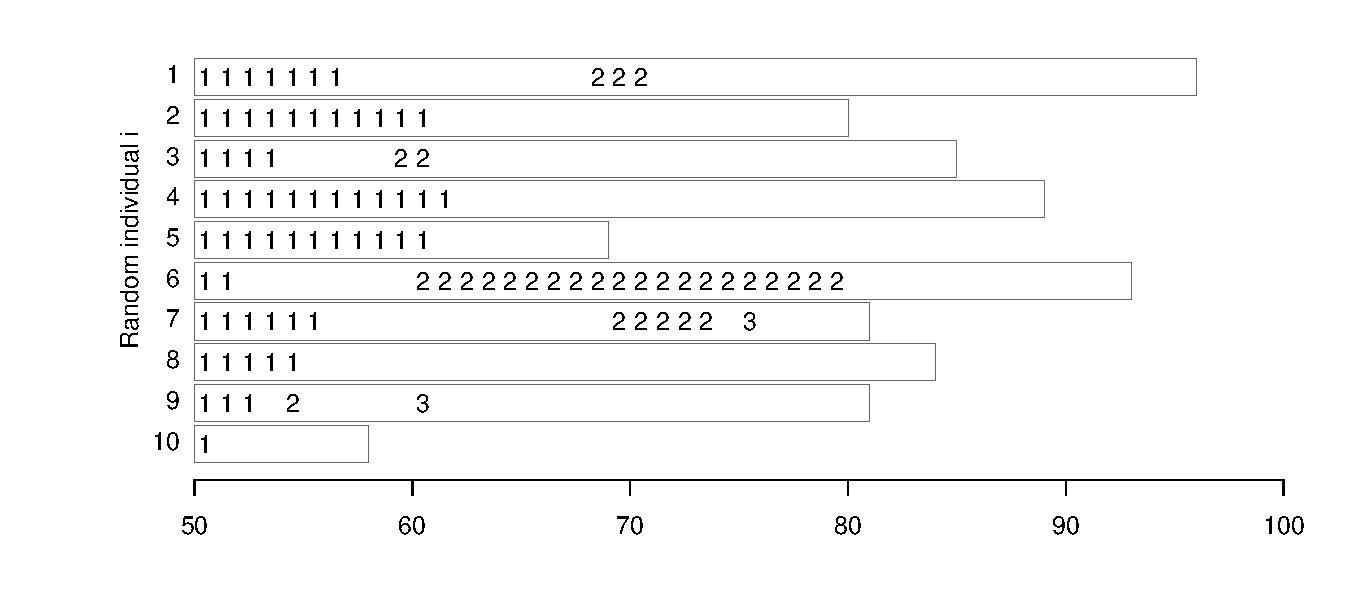
\includegraphics[scale=.5]{Figures/Seq10ordUp.pdf}
\end{subfigure}

\begin{subfigure}{\textwidth}
\caption{Employment episode order, decreasing.}
\label{fig:orderdown}
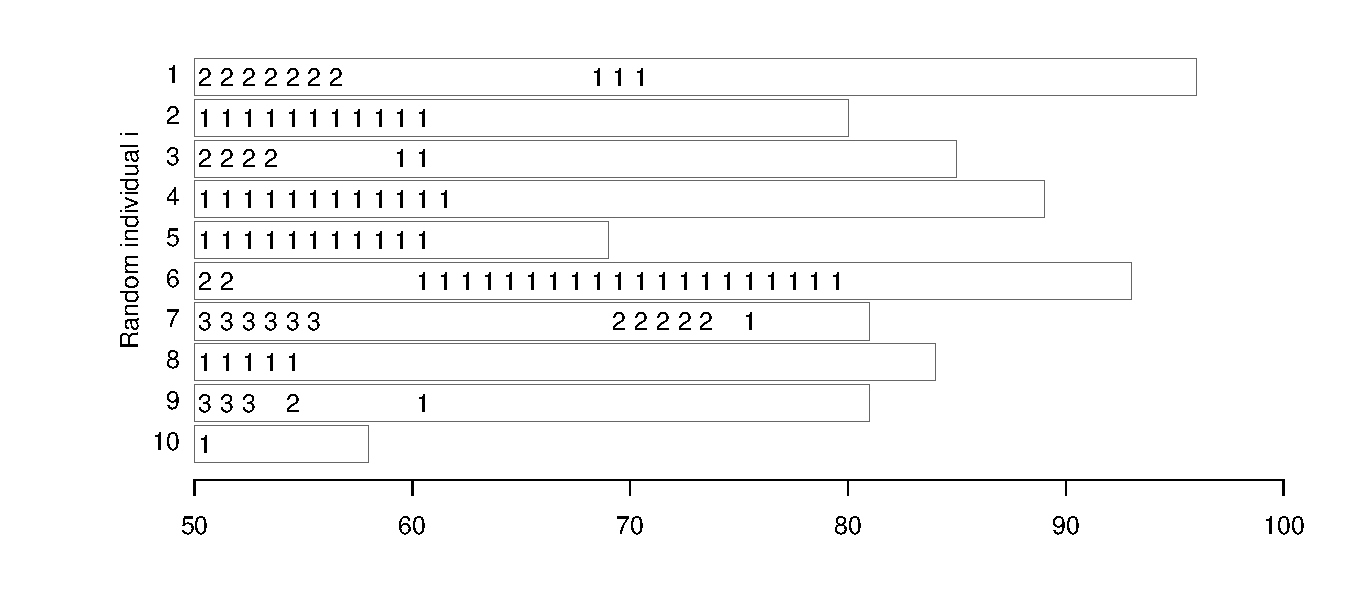
\includegraphics[scale=.5]{Figures/Seq10ordDown.pdf}
\end{subfigure}

\end{figure}


\FloatBarrier
\subsection{Alignment}
Episodic clock values are aggregated according to some
structuring criteria. In all previous figures, the structuring criteria was
chronological age, which is how data were generated in the first instance. To
introduce a term, these figures are \emph{left-aligned} on the event of birth.
This is the most common default alignment in social and medical sciences, but other choices may be more
compelling for particular questions.

For late-life processes, birth is usually a long ways off, and empirical
regularity may be be found with respect to other alignment criteria. Aligning lifelines requires
two choices: 1) a reference moment or anchoring \emph{event} must be selected,
and 2) the alignment direction must be chosen. A reference event could be any instance of
entry, exit, or other compelling anchor point, such as a spell midpoint-- ergo
such events likely relate to episodes.
For repeated events, the choice of anchoring episode could itself follow a
regular criterion, such as first, last, or longest episode. The \emph{direction} of
alignment could be left, right, center, or perhaps something else.

Aggregated patterns
would certainly turn out different if we were to right-align on the moment of death, per Figure~\ref{fig:seq10death}.
This particular realignment doesn't seem so compelling for the
demonstrated process, but I suppose it would be
illuminating for health states and the sequence of events leading up to death.

Figure~\ref{fig:alignment} shows a set of four alignment selections out of the
many possible choices. Figure~\ref{fig:firstretire} left-aligns on
entry to \emph{first} retirement (if any). One could also choose last, longest,
or some other episode of retirement, or of course right-align on exit.
Figure~\ref{fig:longinactleft} left-aligns on entry into each individual's
longest spell of inactivity, whereas Figure~\ref{fig:longinactright} right-aligns on exit from
the same spell.

 \begin{figure}[ht!]
\centering
\caption{The sequences from Figure~\ref{fig:seq10} under a variety of alignment
types.}
\label{fig:alignment}

\begin{subfigure}{\textwidth}
\centering
\caption{Right-aligned on death.}
\label{fig:seq10death}
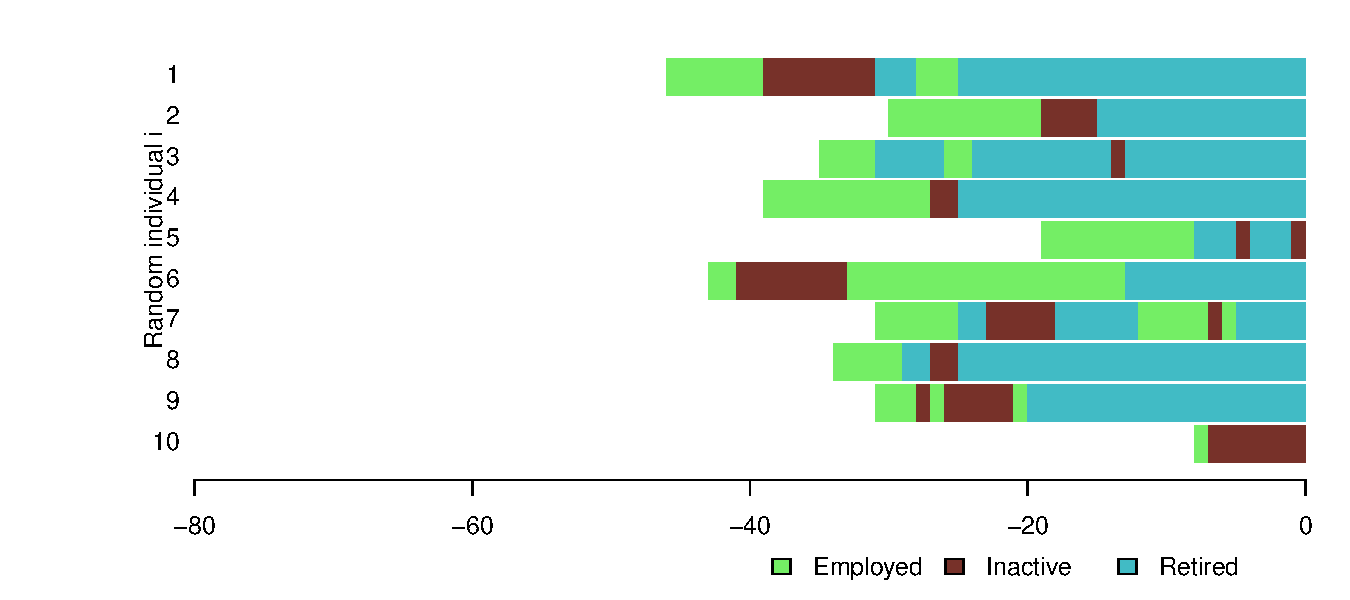
\includegraphics[scale=.5]{Figures/Seq10deathalign.pdf}
\end{subfigure}

\begin{subfigure}{\textwidth}
\centering
\caption{Left-aligned on \emph{first} retirement.}
\label{fig:firstretire}
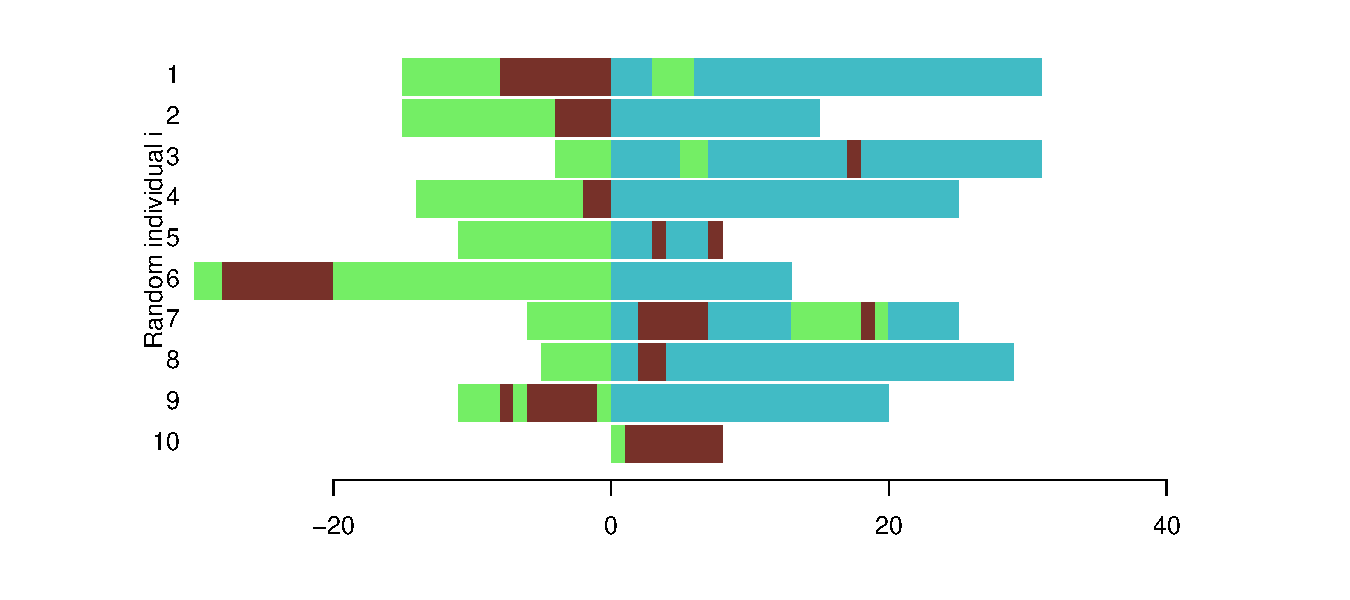
\includegraphics[scale=.5]{Figures/Seq10firstretirealign.pdf}
\end{subfigure}

\begin{subfigure}{\textwidth}
\centering
\caption{Left-aligned on entrance to \emph{longest} spell of inactivity}
\label{fig:longinactleft}
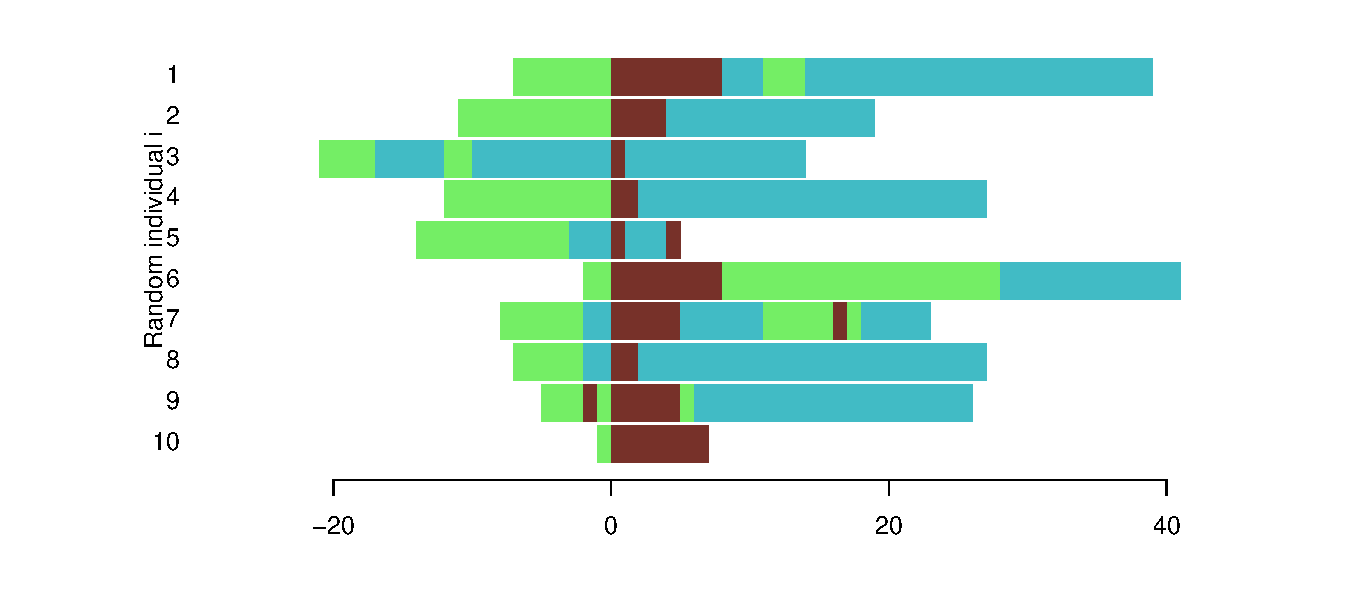
\includegraphics[scale=.5]{Figures/Seq10inactlongleft.pdf}
\end{subfigure}

\begin{subfigure}{\textwidth}
\centering
\caption{Right-aligned on exit from \emph{longest} spell of inactivity}
\label{fig:longinactright}
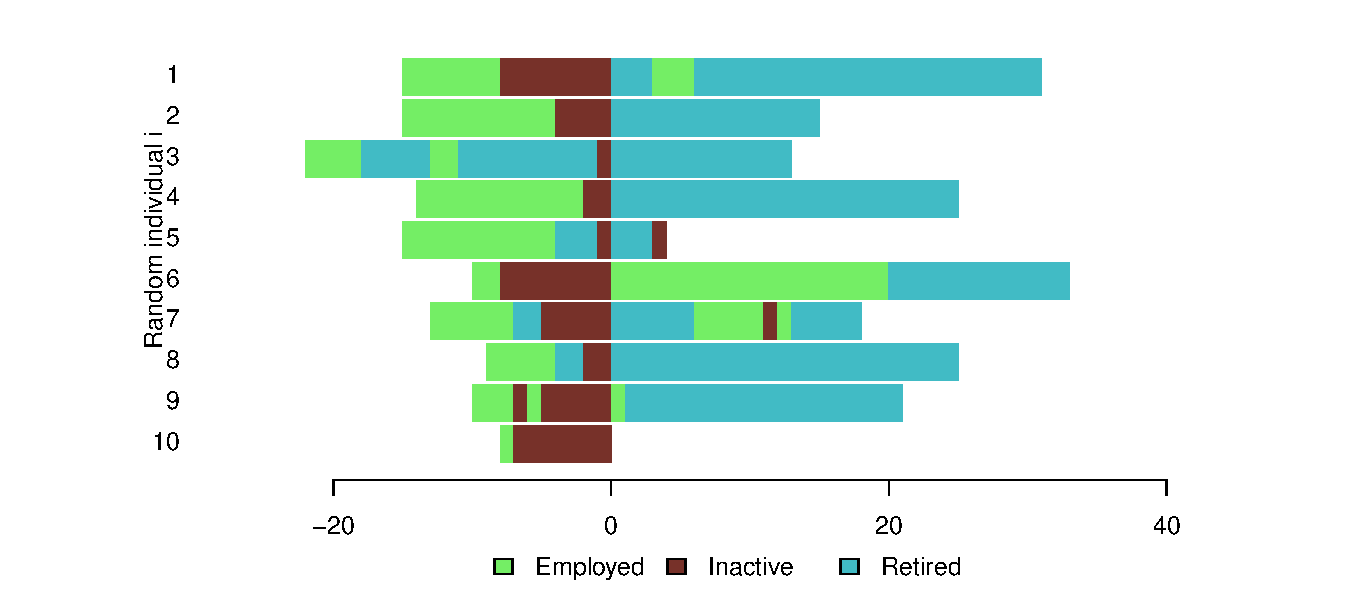
\includegraphics[scale=.5]{Figures/Seq10inactlongright.pdf}
\end{subfigure}

\end{figure}

The purpose of realigning is to bring transitions into focus. We do not showcase
\emph{sorting} in this treatment, as this is another can of worms. Rather, here
we would like to operate on aggregations of individual sequences, in which case
between-individual sorting is unimportant. We'd still like to make statements
about population-level characteristics.





\FloatBarrier
\singlespacing
\bibliographystyle{plainnat}
  \bibliography{references} 
\end{document}
